\chapter[Réflexion]{Première réflexion sur le remote shell}
Pour l'IDE, je prends Code::Blocks. Pas forcément le mieux (et clairement pas un choix de coeur tellement je le trouve laid), mais habituellement, pour du C, je ne prends pas de véritable IDE (Sublime Text *tousse*), donc j'ai envie de changement. Le Makefile est fourni, et le programme s'éxécute dans le terminal, donc je n'ai pas de réel besoin des fonctionnalités de ce programme.
\\\\
Concernant le Remote Shell, l'idée actuelle est de créer un processus par connexion SSH, qui exécutera les commandes qu'il reçoit dans son STDIN. La question étant : est-ce faisable ? La ligne de commande est-elle habituellement donnée via STDIN ?
\\\begin{figure}[!htp]
\centering
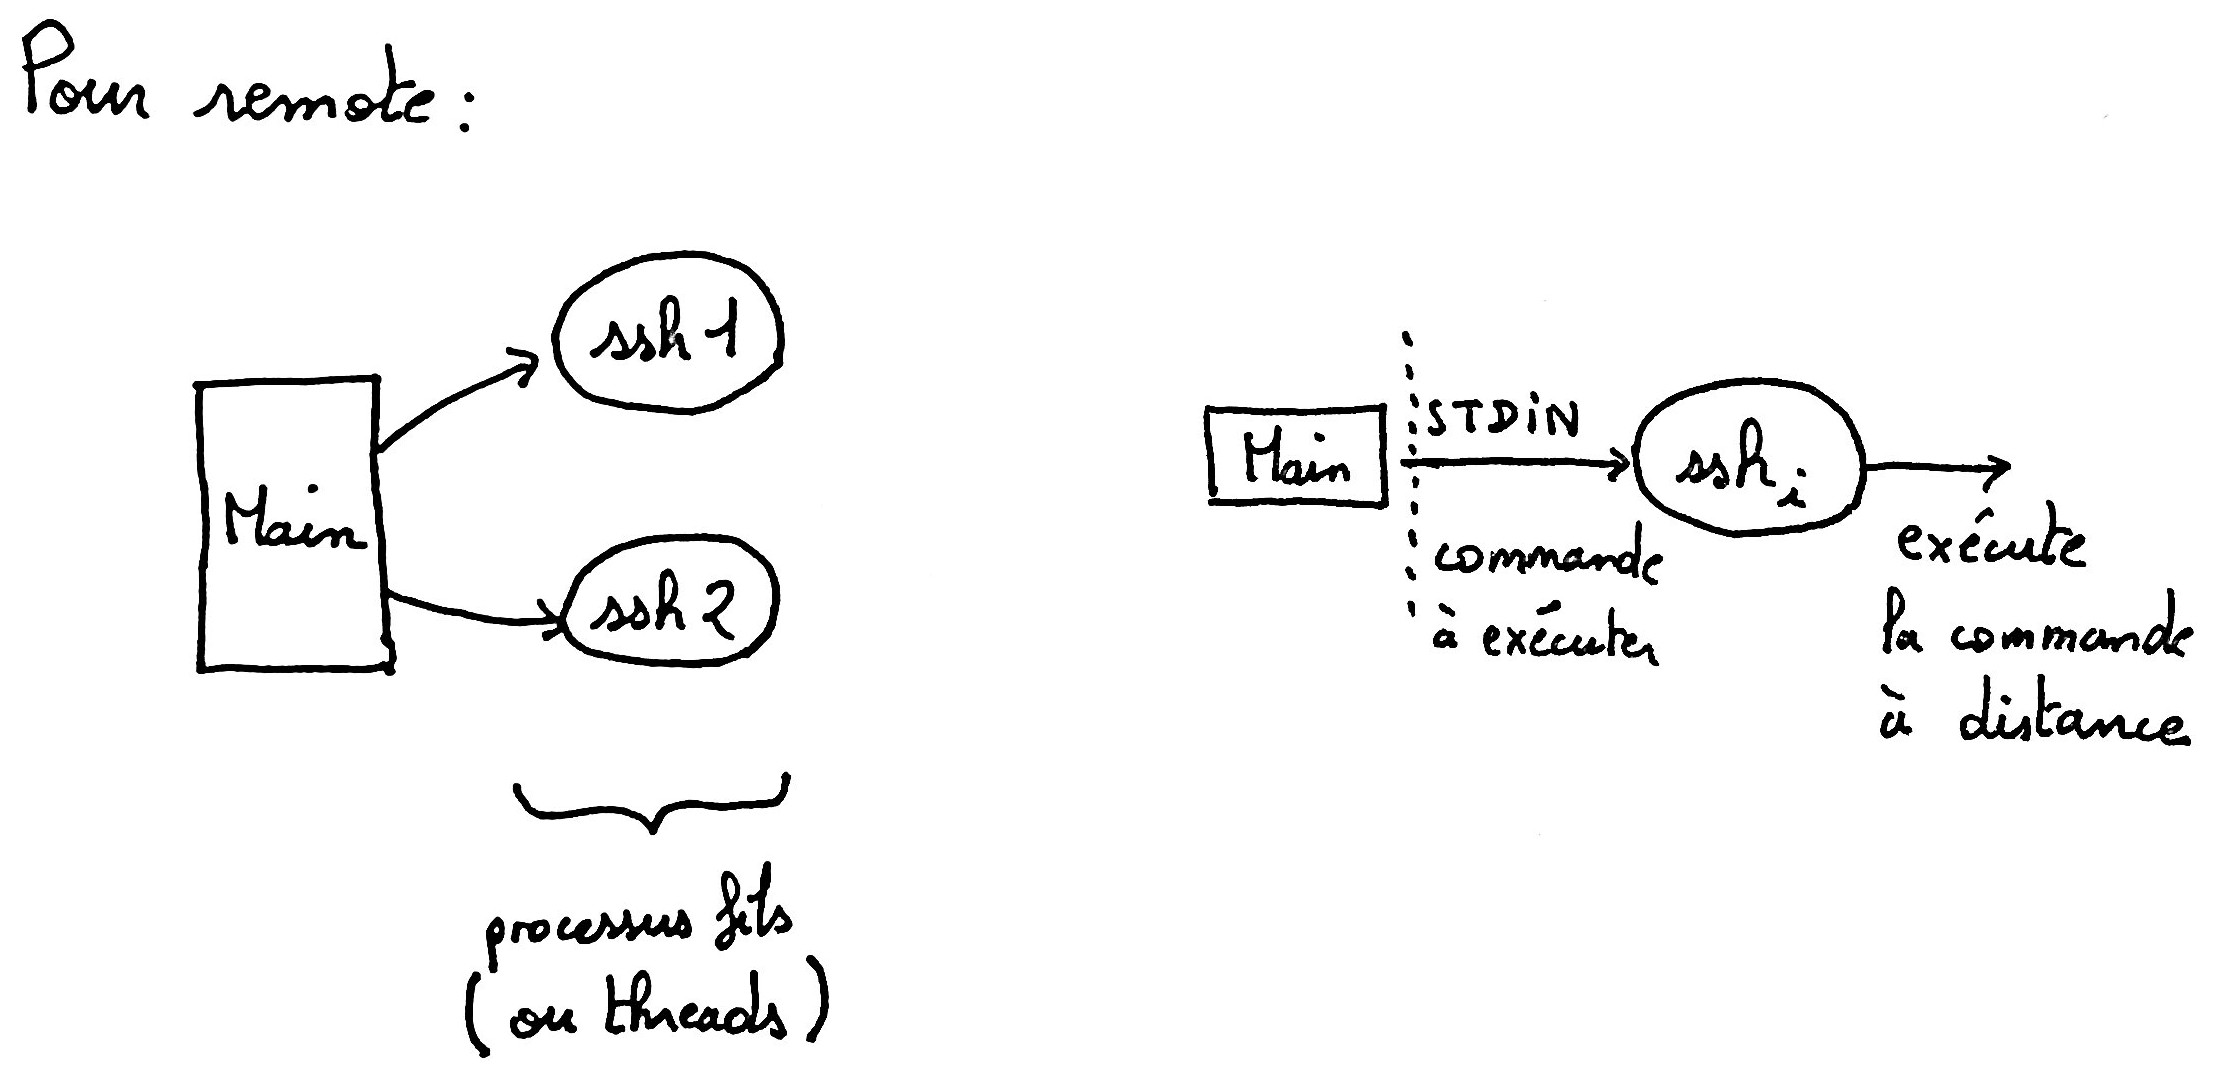
\includegraphics[width=400pt]{Axel-02_Manuscrit1.jpg}
\end{figure}
\\\begin{figure}[!htp]
\centering
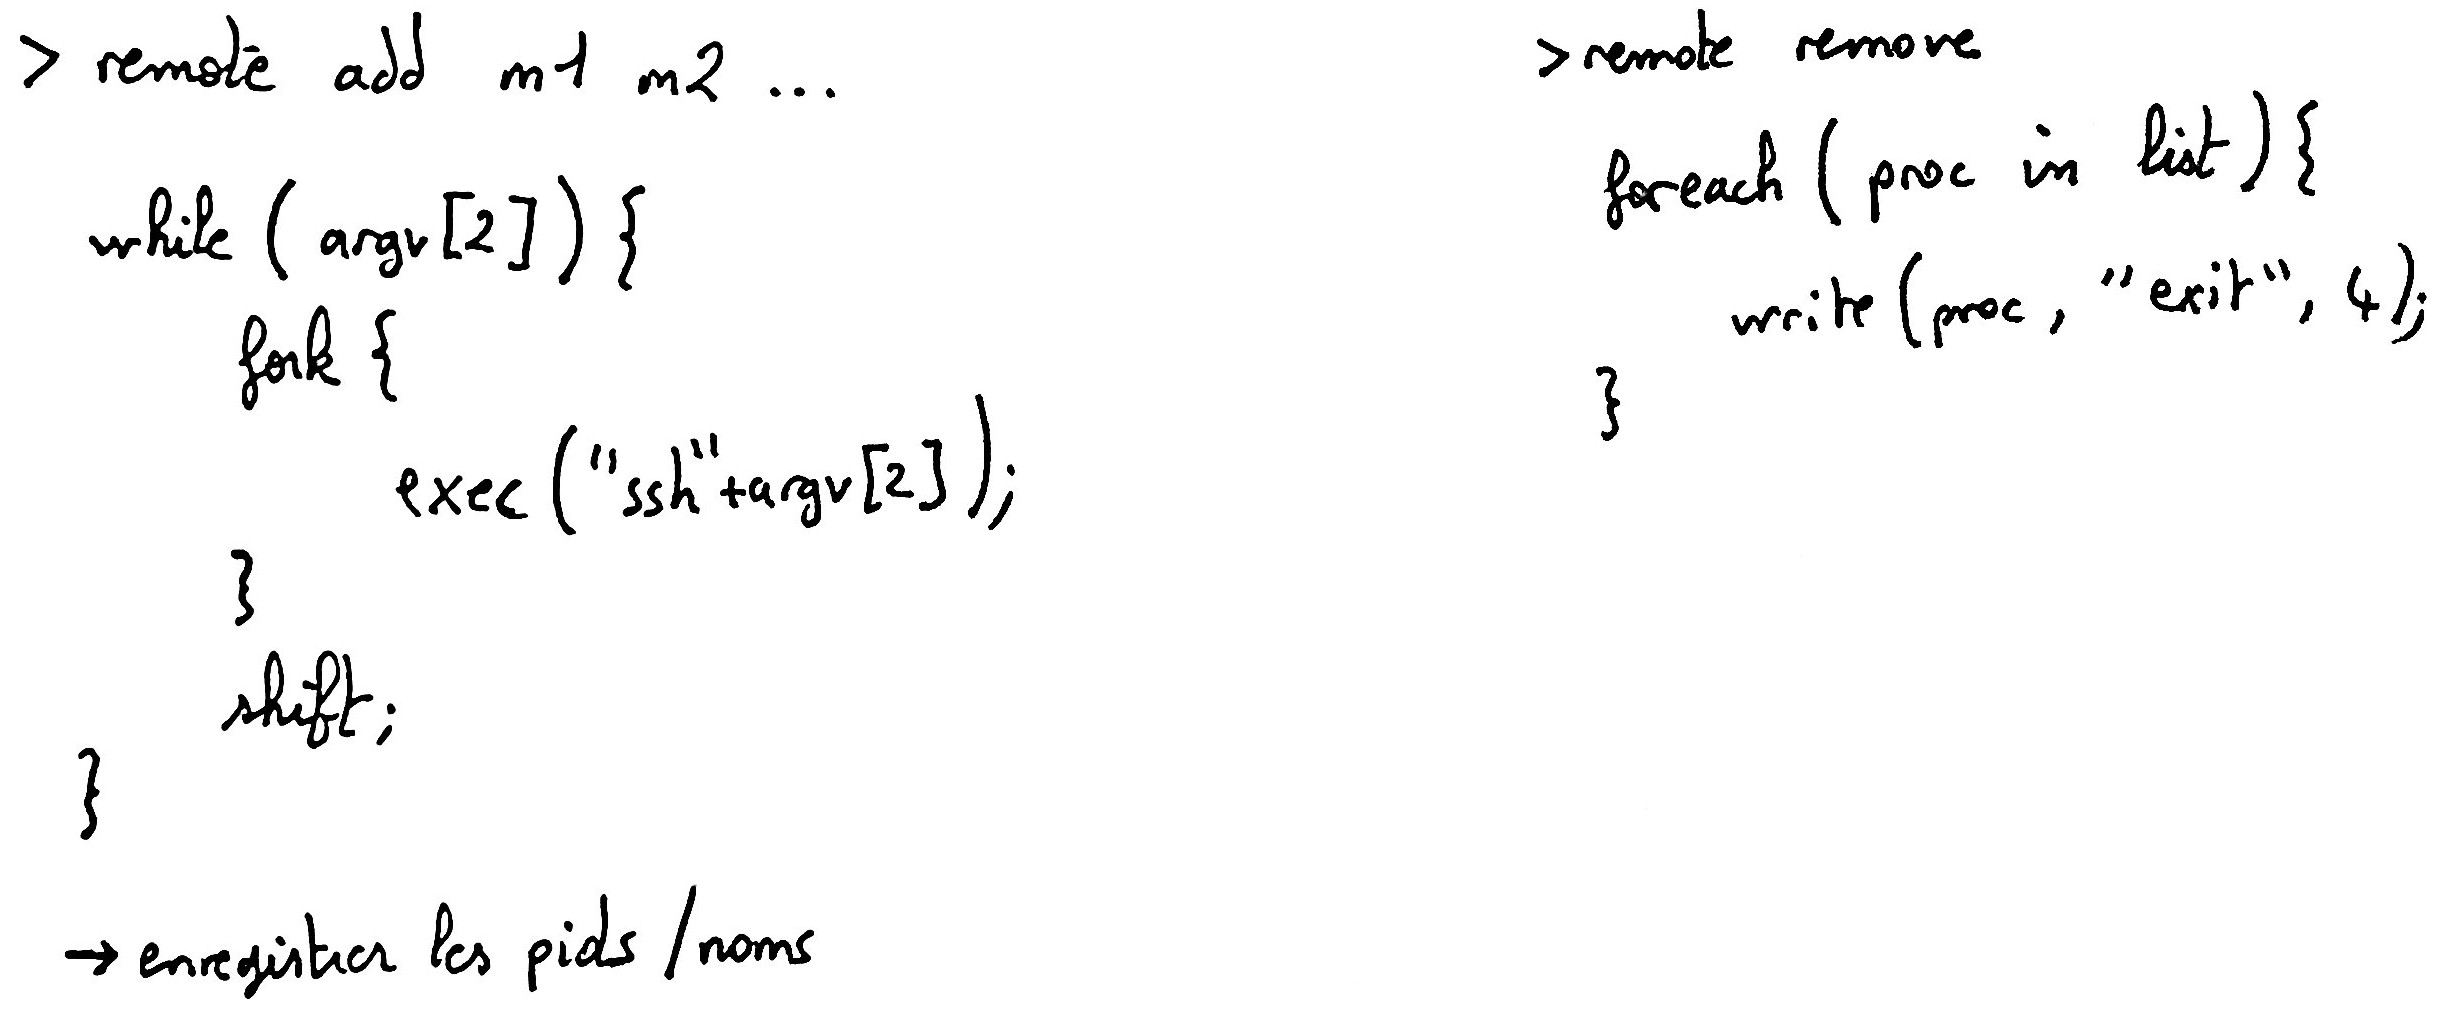
\includegraphics[width=400pt]{Axel-02_Manuscrit2.jpg}
\end{figure}
\\\begin{figure}[!htp]
\centering
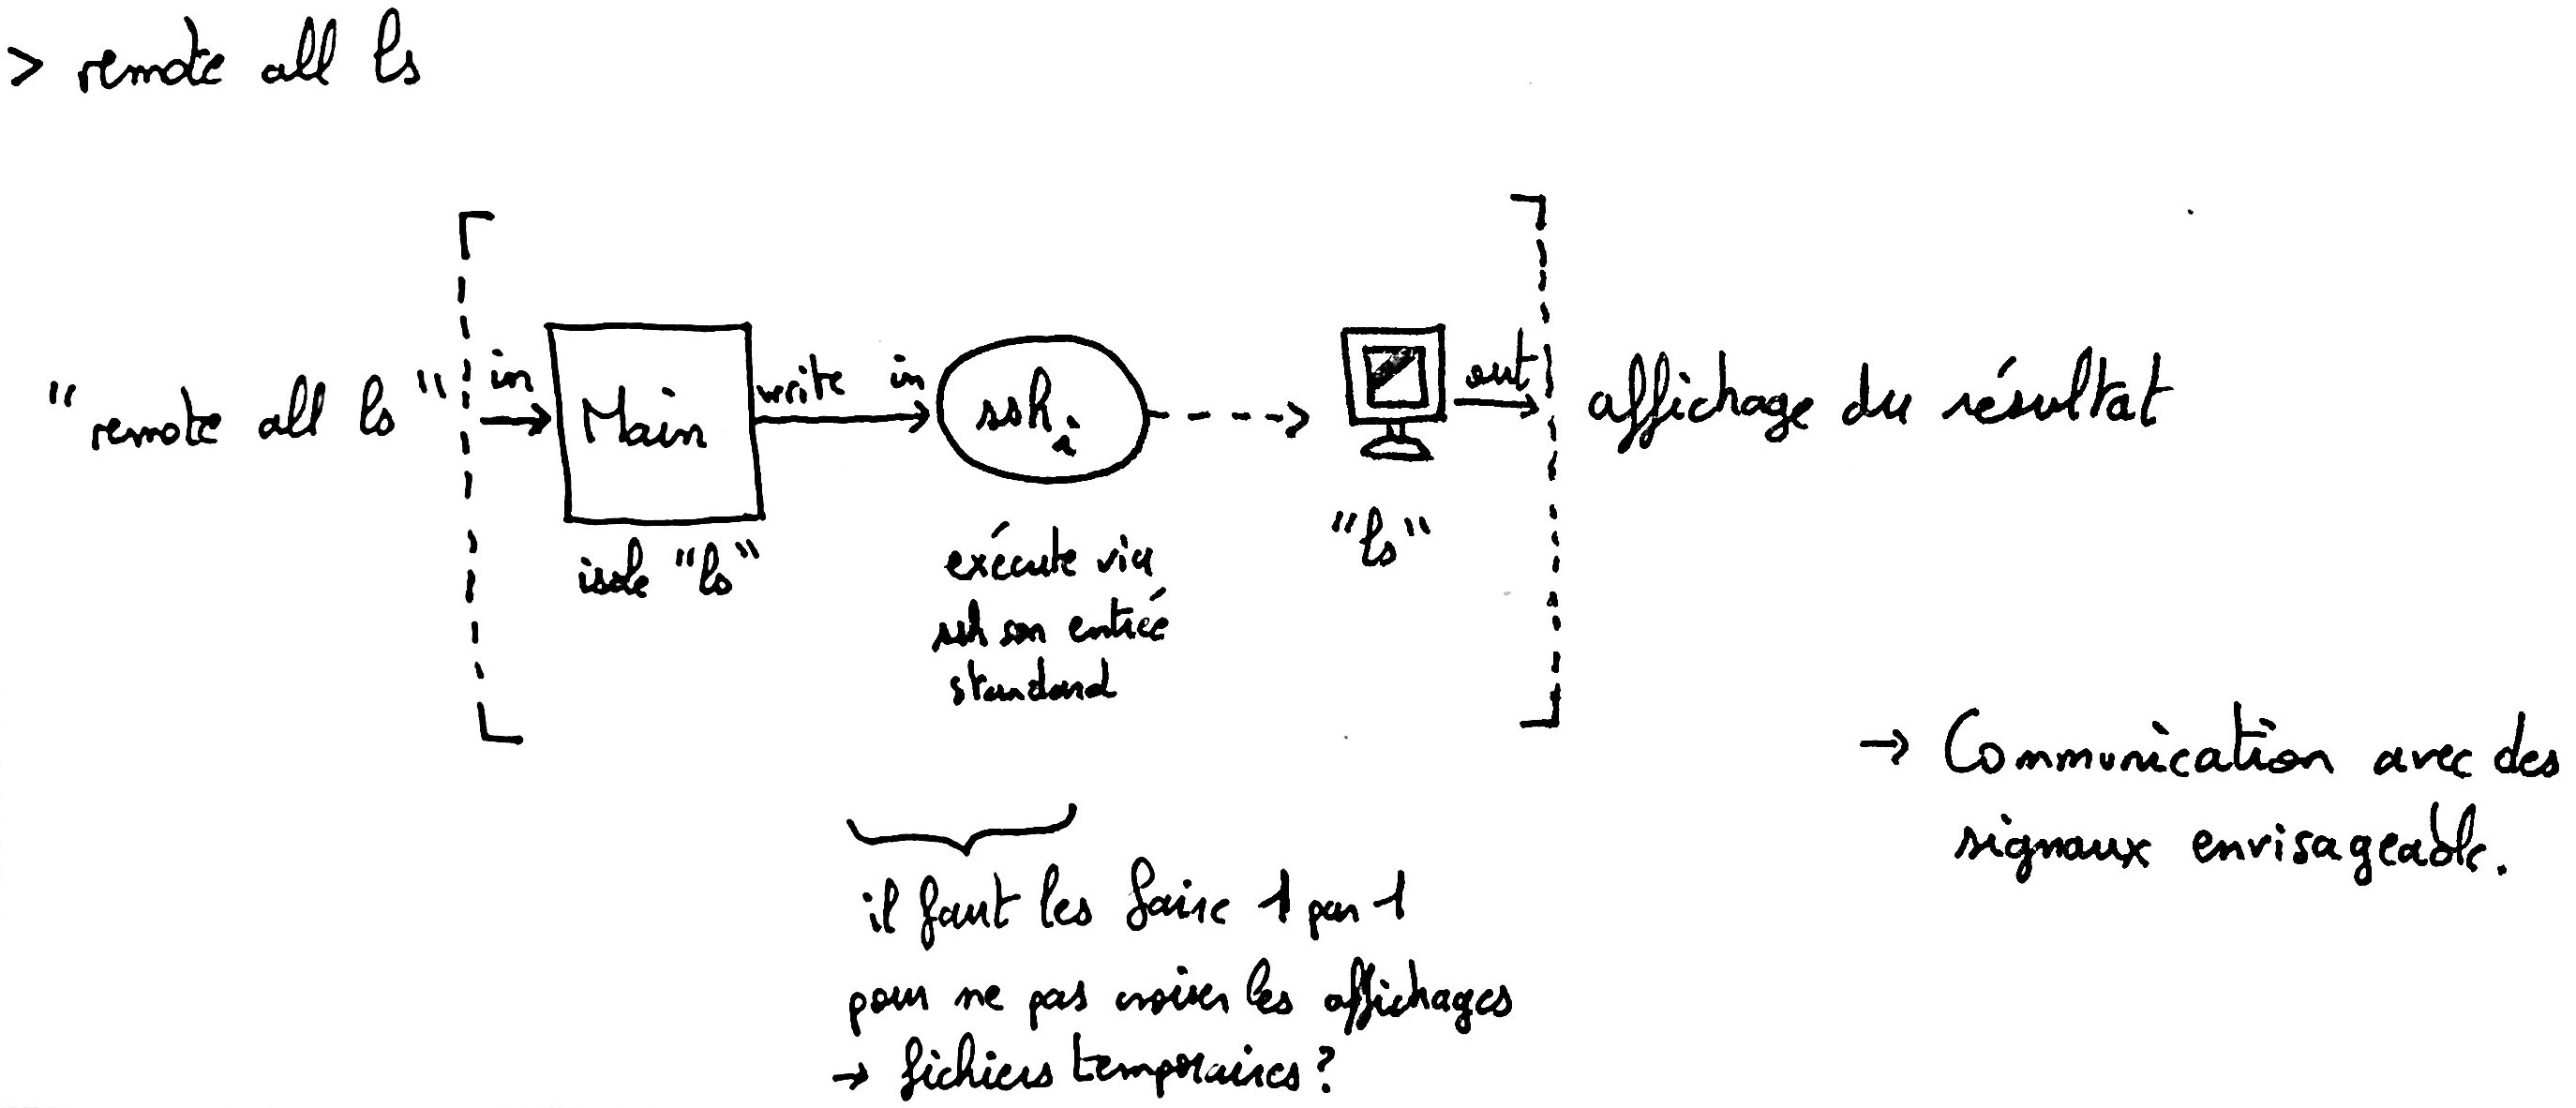
\includegraphics[width=400pt]{Axel-02_Manuscrit3.jpg}
\end{figure}
\\La solution qui me semble sous-entendue dans le sujet est d'exécuter à chaque fois "ssh host cmd". Ça me paraît vraiment lourd, et ça ne conserve pas les connexions. De même, comment ouvrir une connexion ssh avec mot de passe au travers de notre processus principal ? On peut rediriger l'entrée vers la sortie, mais comment savoir à quel moment redonner la main à notre mini-shell ?
\\\\
La commande mkfifo semble intéressante pour cela. Elle crée une file nous permettant d'écrire dans le STDIN d'un processus : "mkfifo myfifo ; ssh host < myfifo ; echo lol > myfifo" permet d'envoyer "lol" dans le STDIN du processus SSH. Ça ressemble grandement à ce que je veux ! Actuellement, ma connexion Internet est prise par les innombrables mises à jour (joie), donc ssh met trop de temps à répondre. Je testerai plus tard. Mais si ça fonctionne, c'est probablement ce qu'on utilisera ! Le seul problème que je peux y voir actuellement, c'est comment créer et conserver notre file. À voir plus tard. De même, l'utilisation d'une file semble aspirer le STDOUT du programme...
\\\\
J'avais oublié à quel point il est agréable de créer un projet versionné via git, et géré par Code::Blocks. Ce sera Sublime Text. Pas particulièrement fonctionnel, mais je m'en sortirai avec ça.
\\\\
Je vais tester en ligne de commande si écrire dans STDIN fonctionnerait.
\\\$> mkfifo fifolol
\\mkfifo: impossible de créer la FIFO «fifolol»: Le fichier existe
\\\\
Oh ? Je pensais que ces files étaient temporaires. J'avais déjà donné ce nom à ma file précédente, quand j'ai découvert cette commande. Effectivement, en lançant ls, je vois que mkfifo crée un fichier fifolol. Je peux le supprimer avec rm. C'est une sorte de "faux pipe" si je puis dire.
\\\\
\$> bash < fifolol \&
\\\$> cd /
\\\$> echo "pwd" > fifolol
\\bash : fifolol : Permission non accordée
\\\\
Oh ? Encore une erreur ? Je n'ai pas les droits sur mon pipe ? Qu'à cela ne tienne : supprimons-le, et recréons-le.
\\\$> mkfifo fifolol
\\\$> bash < fifolol \&
\\\$> cd /
\\\$> echo "pwd" > fifolol
\\bash : fifolol : Permission non accordée
\\\\
MAIS QUEL CON ! Je fais un cd, puis je nomme fifolol... Qui n'est donc plus là. Quel idiot.
\\\$> echo "pwd" > \textasciitilde/fifolol
\\/home/seiken
\\\\
MAGNIFIQUE ! ÇA FONCTIONNE ! Bon, le bash s'est terminé une fois la commande exécutée. Mais on peut outrepasser ce problème avec tail :
\\\$> tail -f fifolol | bash \&
\\\\
Là, je peux envoyer des commandes à bash à l'infini. C'est juste. TROP. GÉNIAL. J'ai presque envie d'arrêter le projet ici, tellement je suis refait. Mais bon. Testons maintenant avec un ssh. Je lance la connexion, puis je tente de lui passer une entrée via un autre terminal.
\\\$> cd -
\\\$> ssh adubroca@jaguar.emi.u-bordeaux.fr < fifolol \&
\\(Deuxième terminal : \$> echo " *** " > fifolol)
\\Pseudo-terminal will not be allocated because stdin is not a terminal.
\\\\
Hum. Embêtant. J'ai tout simplement essayé d'envoyer mon mot de passe via la file (procédé hautement sécurisé, vous en conviendrez. Je l'ai au moins censuré dans ce rapport). Mais le seul moyen de l'entrer, c'est un terminal. Part-on du principe que nous n'avons pas de mot de passe à entrer ? Après tout, au CREMI, puisque nous sommes authentifiés, nous n'en avons peut-être pas besoin. Mais cela rendrait ce projet futile, à mon avis. Bref.